\documentclass[Main]{subfiles}
\begin{document}

\subsection{SekvensDiagrammer}

\subsubsection{Use Case 1 -- System initialisering}

\begin{figure}[H]
\centering
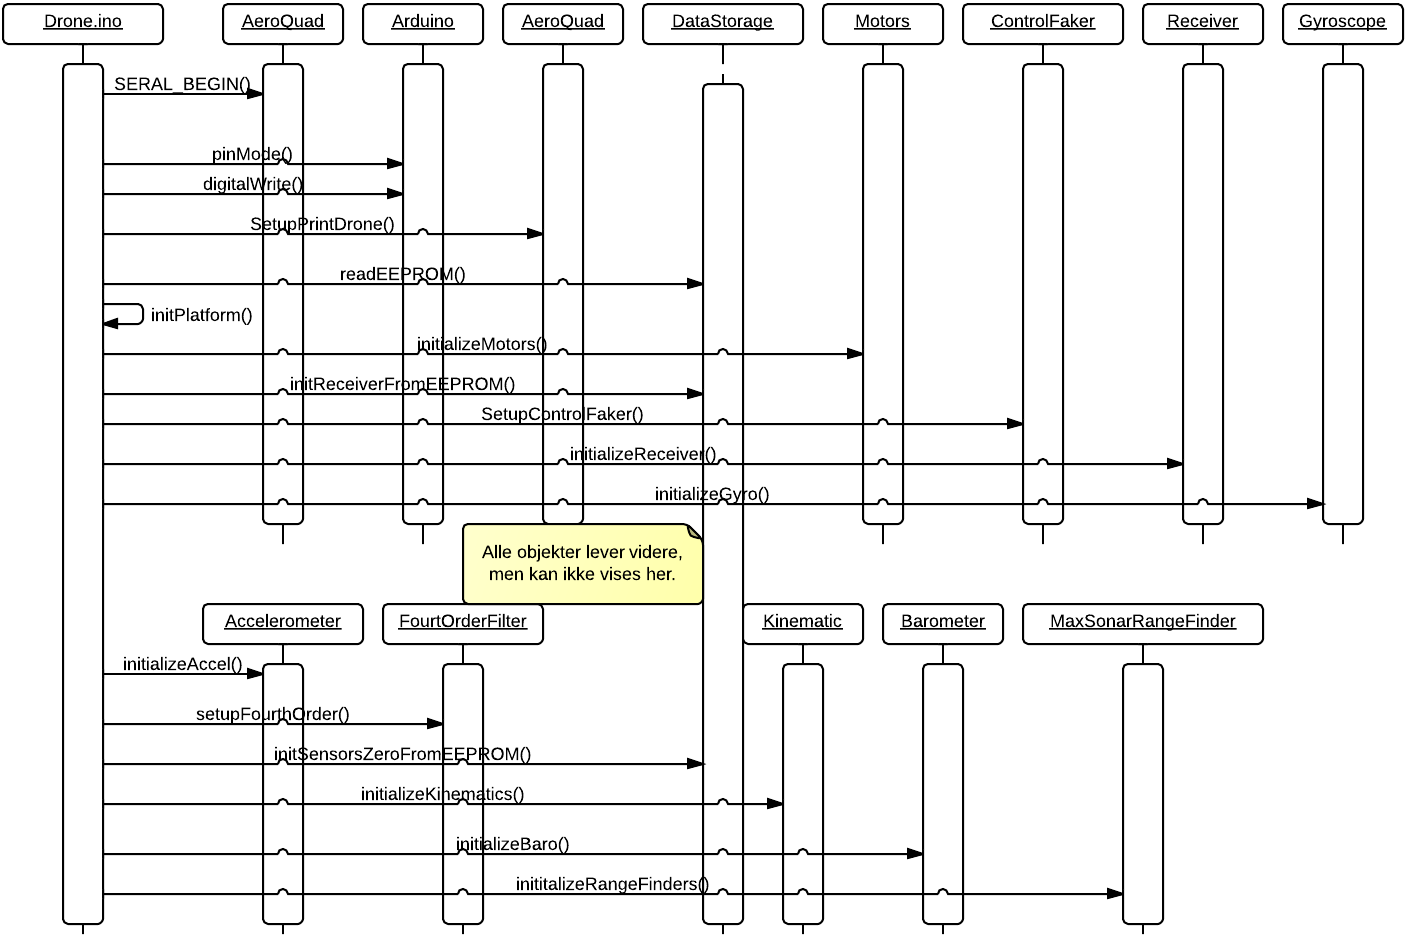
\includegraphics[angle=90, scale = 0.41]{SekvensInit}
\caption{Init af drone}
\label{Fig:SekvInit}
\end{figure}

På Figur \ref{Fig:SekvInit} ses de kald der foretages, når dronen starter op første gang den får strøm.
Efter initieringen startes Arduino's \code{loop()}-funktion, der kører i ring til strømmen afbrydes, som vist på Figur \ref{Fig:SekvDroneHz}.


\begin{figure}[htbp]
\centering
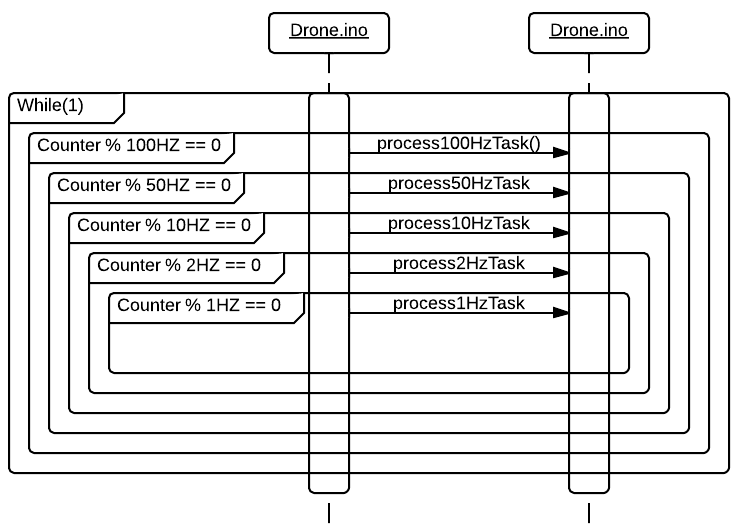
\includegraphics[width = 0.7\textwidth]{DroneLoop}
\caption{Schedulering i \code{loop()}-funktionen}
\label{Fig:SekvDroneHz}
\end{figure}

Input til, hvordan dronen skal flyve, bliver registreret i \code{50HzTask()} og er illustreret på Figur \ref{Fig:50Hz}.

Når kalibreringen og sikkerhedstjekket er kørt igennem, nulstilles \code{Receiver}'ens lokale værdier, samt \code{ControlFaker}'ens og \code{Decision}'s lokale værdier.
Nu er dronen klar til at flyve.

Herefter vælges hvilket program der skal køres, der pga. nulstillingen er default-programmet, vil få dronen til at spinne med minimal hastighed. hvilket først læser det aktuelle programs data, sætter hastighed og derefter eksekverer dataene.

XXX What 


\begin{figure}[H]
\centering
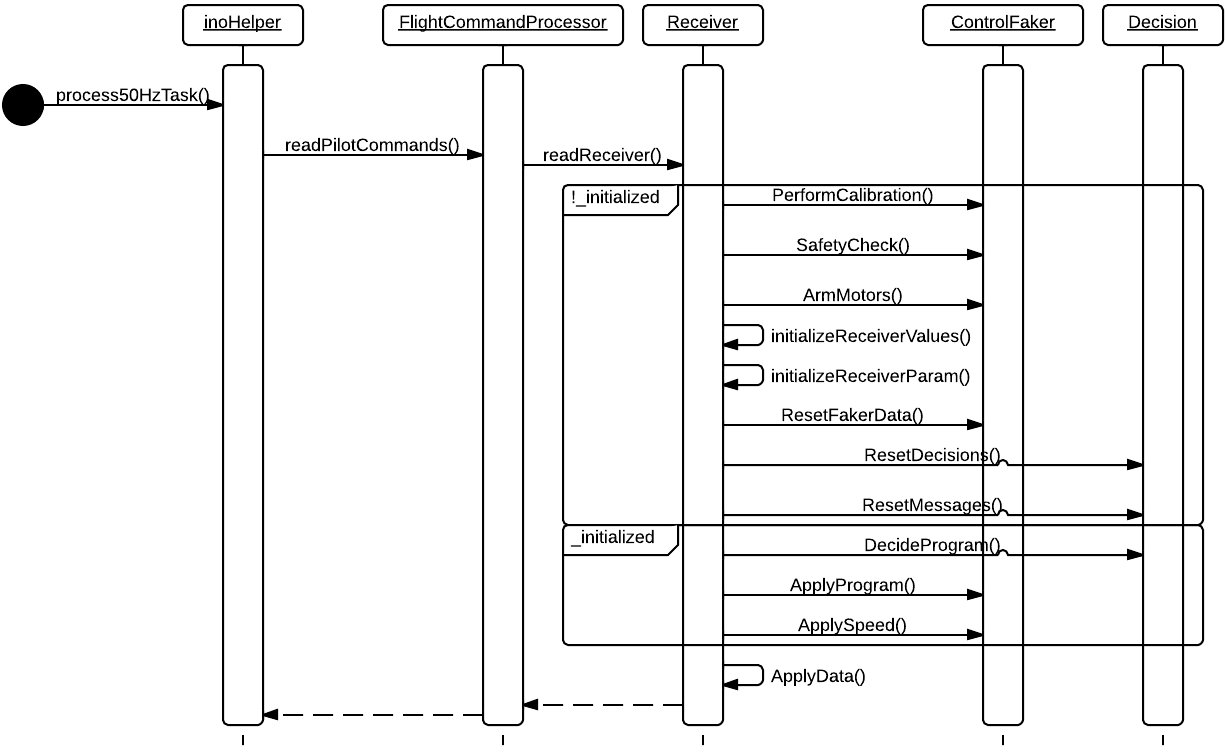
\includegraphics[width = \textwidth]{50HzProcess}
\caption{50 Hz processen. }
\label{Fig:50Hz}
\end{figure}




\newpage
\subsubsection{Use Case 2 -- Programvalg}
Når brugeren af systemet vælger et program, sendes signalet fra fjernbetjeningen til dronens radiomodtager, der læses af \code{DecideProgram()} (fra Figur \ref{Fig:50Hz}) og er illustreret på Figur \ref{Fig:SendProgram} ved funktion nummer 4.

\begin{figure}[H]
\centering
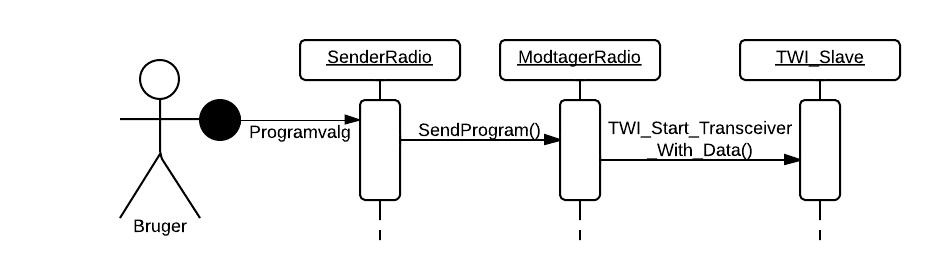
\includegraphics[width = \textwidth]{SendProgram}
\caption{Skriv til radio.}
\label{Fig:SendProgram}
\end{figure}


\newpage
\subsubsection{Use Case 3 -- Sonaradvarsel}
Når dronen flyver kan de 3 sonarsensorer, der sidder foran den, registrere hvor langt der er til nærmeste objekt i en kegle 67$^{\circ}$ (se Afsnit \ref{Sec:Sonar}).
Såfremt de registrerer noget (på et gennemsnit af de seneste to målinger), vil et flag blive sat, hvilket checkes for i \code{4: DecideProgram()} (fra Figur \ref{Fig:SendProgram}), hvorefter dronen vil reagere på alle kombinationer der er af disse input (se Tabel \ref{Tab:SonarAdvarsel}).


\begin{figure}[H]
\centering
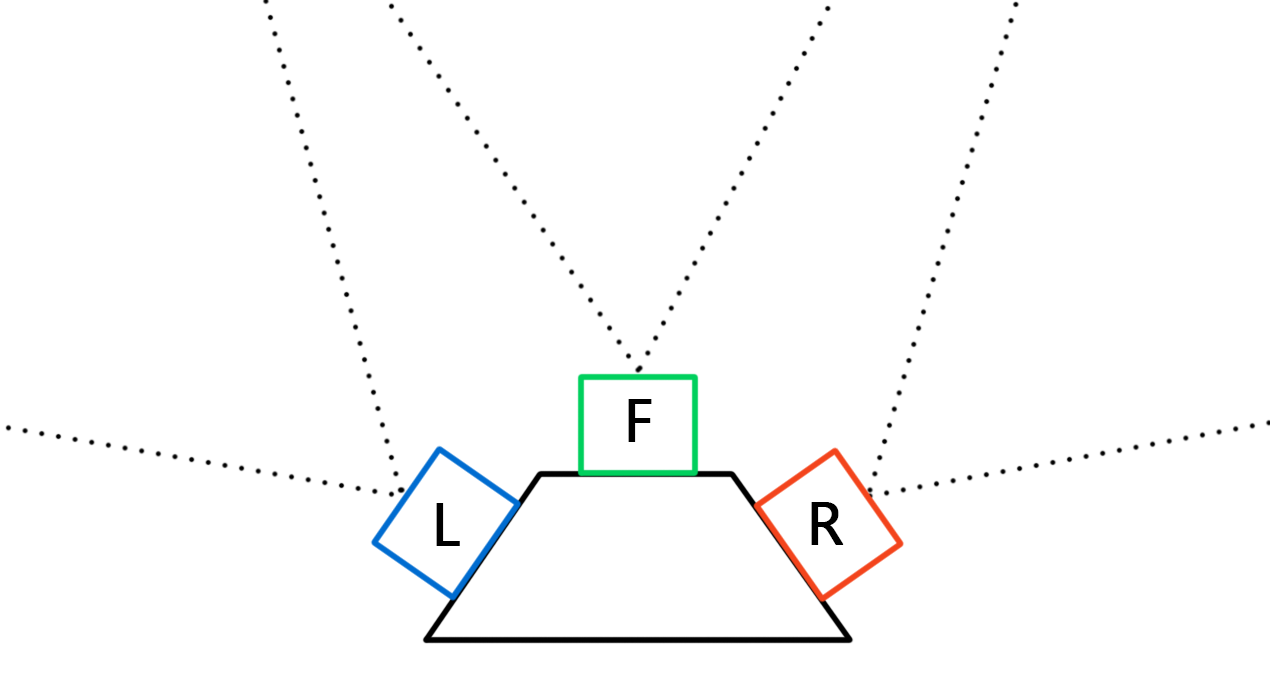
\includegraphics[width = 0.65\textwidth]{SonarSketch}
\caption{Skitse af sonarmodulet. Venstre (blå), front (grøn) og højre (rød).}
\label{Fig:SonarSketch}
\end{figure}

\begin{table}[H]
\centering
	\begin{tabular}{l l}
	\hline Kombination & Reaktion
	\\ \hline 
	L+F+R & Stop og roter til venstre \\
	L+R & Stop og roter til venstre\\
	L+F & Stop og roter til højre\\
	L & Roter til højre\\
	F+R & Stop og roter til venstre\\
	F & Stop og roter til højre\\
	R & Roter til venstre\\
	Intet & Foretag ingen ændring \\ \hline
	\end{tabular}
\caption{Kombinationsmuligheder ved sonaradvarsel.}
\label{Tab:SonarAdvarsel}
\end{table}

\newpage
\subsubsection{Use Case 4 -- Maks. spin stop}
Use Case 4 aktiveres af dronen, hvis en af dronens propeller skal spinne med værdien over 2000 RPM (hvilket også er dens maksimale spinhastighed).
Dette scenarie finder kun sted, såfremt dronen forsøger at rette sig selv op efter den er fløjet ind i noget og/eller en propel er blev beskadiget og derfor ikke retter dronen op, som den ellers burde.

Beregningerne foretages 100 gange i sekundet og er vist på Figur \ref{Fig:100HzProcess}, hvor systemet kalder funktionen \code{2: CalculateFlightError()}, der beregner hvor meget dronen skal justere sig på x- og y-aksen for, at holde sig vandret i luften.
Når dette er gjort anvendes de udregnede værdier i funktionen \code{7: ApplyMotorCommand()}.

\begin{figure}[H]
\centering
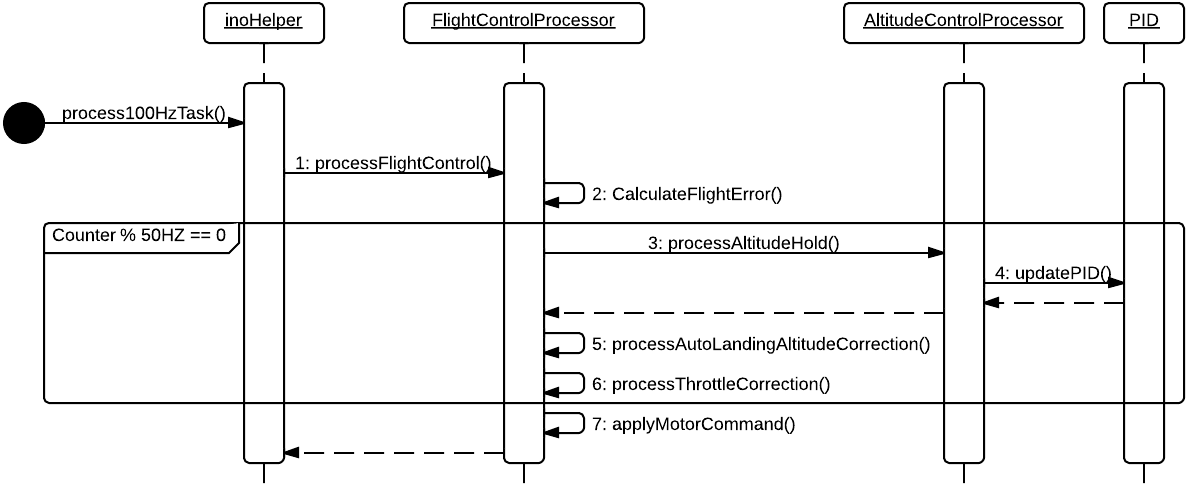
\includegraphics[width = \textwidth]{100HzProcess}
\caption{\code{100HzProcess}-funktionen fra klasse \code{InoHelper}}
\label{Fig:100HzProcess}
\end{figure}

Når PID-ændringer virker som de skal og bliver anvendt på dronen, ser det ud som på Figur \ref{Fig:PID-outcome}. Outputtet er den værdi der sendes til motorerne.

\begin{figure}[htbp]
\centering
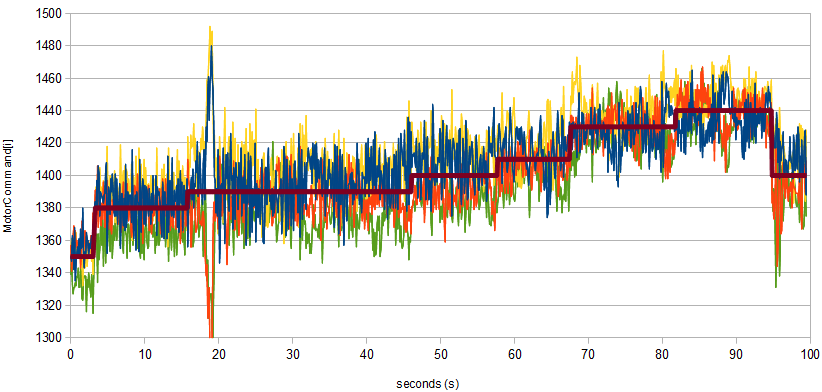
\includegraphics[width = \textwidth]{PID-outcome}
\caption{PID'ens effekt på de fire motorer vist med forskellige farver, samt det de skal ramme (markeret med fed mørk rød).}
\label{Fig:PID-outcome}
\end{figure}

Når PID-ændringerne til gengæld ikke virker, ser det ud som på Figur \ref{Fig:PID-fail}.
Det ses, at værdierne pludselig springer langt væk fra, hvad de burde være, hvilket er årsagen til at grænsen blev indført.

\begin{figure}[htbp]
\centering
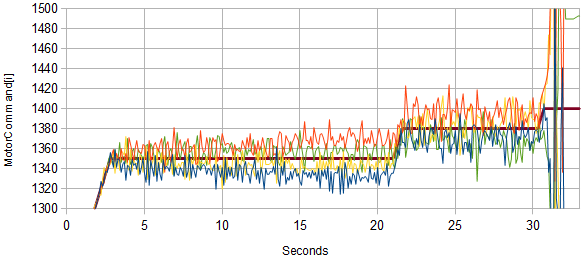
\includegraphics[width = \textwidth]{PID-fail}
\caption{PID'ens effekt på de fire motorer når en propel er beskadiget.}
\label{Fig:PID-fail}
\end{figure}




\end{document}